\chapter{Success Prediction Model Analysis}
\label{chapter:analysis}
In this chapter, we present our methodology and experimental results related to
the prediction model presented in Chapter~\ref{chapter:model}. We begin with
the methodology in Section~\ref{sec:method}, which presents our approach for
assessing the predictive model's accuracy according to different types of input
features. Then, in Section~\ref{sec:featureselection}, we present our approach
for analyzing all 121 features from Table~\ref{tab:features} in order to select
the ones that show a \textit{greater dependence}\footnote{Dependence is the
statistical relationship between two sets of data.} with movie success.
Finally, in Section~\ref{sec:results}, we present and discuss results, showing
they confirm the main hypothesis of this work, which is: \textit{In a
multivariate predictive analysis of movie success, using many topological
features from teams leads to a more accurate analysis.}

\section{Methodology}
\label{sec:method}
Choosing a single split of train/test sets might produce poor experimental
results, because the train and test sets could be selected in a biased
way~\citep{mohri2012foundations}. To avoid this problem, we perform
\textit{K-fold Cross Validation} with $K = 5$.  The selection of $K$ was made
such that it effectively controls the bias while it generates large folds that
are more heterogeneous. For each cross validation, the movies are randomly
split into five distinct groups, and five train/test cycles are performed. Each
time, one of the groups is chosen to be the test group and the other groups are
used for training the regression model. In each train/test cycle, the
coefficient of determination\footnote{Throughout this chapter, the coefficient
of determination (denoted as \textbf{$R^2$}) is used to assess how well the
different regression models are predicting movie success according to their
given inputs.} is computed by evaluating the model using the respective test
set. This gives five $R^2$ values for each run. We consider the mean of these
values as the result of the cross-validation execution.

For each evaluation, it is important to ensure that the special five folds were
not randomized in a biased way. Hence, when evaluating a model, we take results
from 30 different \textit{5-fold cross validation} executions. We then
calculate the mean and confidence intervals ($\alpha$ = 95\%) from such runs as
the model's final score.
 
If the distribution of votes and gross are highly skewed, forming a power law 
(few movies with most votes and gross, see Figure~\ref{fig:hist_success}), 
there is a high probability that either no or an insufficient amount of 
high-performing movies will be present in several randomized folds. Such skewness 
might favor the formation of biased train/test sets. This could impair the model's 
ability to recognize higher performing movies and thus compromise its accuracy.

To account for this phenomenon, we attempted under-sampling the number of
movies with lower levels of success in the training sets. However, following
experimental evaluation showed this does \textit{not} improve regression
accuracy.  Hence, we choose to generate \textit{balanced} train/test folds.
Using \textit{balanced} folds, train and test sets of movies are grouped in a
way that ensures groups have similar distributions of movies among each of the
three performance groups ($G_1$, $G_2$ and $G_3$ as defined in
Table~\ref{tab:success_groups}). Moreover, all train/test folds are still
generated in a random fashion.

Finally, Algorithm~\ref{algo:predictor} provides an overview of all major steps
and processes involved in the experiments. Briefly, it shows all steps starting
from the raw data all the way to a trained movie success prediction model and
its performance.

\begin{algorithm}[tb]
 \SetKwInOut{Input}{input}\SetKwInOut{Output}{output}
 \Input{Raw IMDb Movie Data}
 \Output{Movie success prediction model}
    $\mathbb{G} \leftarrow$ [~] \tcc*[r]{producers' graph}
    movie\_map $\leftarrow$ [~] \tcc*[r]{movies with features}
    $filter\_by\_votes(\mathbb{M}, minimum\_votes)$\;
    $sort(\mathbb{M}, release\_date)$\; 
    \ForEach{m $\in$ $\mathbb{M}$}{
        $\mathbb{G}.update(\mathbb{P}m)$  \tcc*[r]{add movie producers}
        \If{$any(\mathbb{P}m \cap \mathbb{G}.giant\_component)$}{
            x $\leftarrow$ $m$.success\_parameters\;
            f $\leftarrow$ calculate\_features$(m)$\;
            movie\_map.add$(m, x, f)$\;
        }
    }
    normalize\_features$(movie\_map)$\;
    add\_product\_of\_features$(movie\_map)$\;
    models $\leftarrow$ [~] 		\tcc*[r]{regression models}
    \For(\tcc*[f]{30 runs}){$i\leftarrow 1$ \KwTo{} $30$}{
        R2,model $\leftarrow$ ramdom\_cross\_validation$(movie\_map)$;
        models.add$([R2, model])$;
    }
    return \{models.mean, models.confidenceInterval\}\;
\caption{Movie Prediction Task}\label{algo:predictor}
\end{algorithm}

\begin{table}[!ht]
\centering
\caption{\label{tab:test_sets}Three test sets for evaluating prediction accuracy.}
\begin{tabular}{@{}lcc@{}}
\toprule
Year Range & Number of Movies & Proportion of complete set \\
\midrule
2008--2013     &~3,317 &~27\% \\
1995--2013     &~9,775 &~52\% \\
1930--2013     &12,250 &100\% \\
\bottomrule
\end{tabular}
\end{table}


\subsection{Predictive Evaluation}
\label{sub:predictive_evaluation}
The methodology for evaluating the prediction model consists in 
splitting the movies in three chronological groups: from 2008 to
2013 (3,317 movies = 27\%), from 1995 to 2013 (9,775 movies = 52\%), and from
1930 to 2013 (12,250 movies = 100\%). We use each group for
training and testing the regression models for each of the three success
parameters. Table~\ref{tab:test_sets} summarizes the three different experiment
sets.

To evaluate how the features that depend on team social characteristics add
predictive power to the model, experimental trials are performed with the same
set of movies $\mathbb{M}$, but using different sets of features. Specifically,
we evaluate the regression model three times by considering: only the
non-topological features, only the topological features and all features.
Finally, we use the coefficient of determination~$R^2$ to assess how well the
regression models are predicting movie success parameters.

\section{Feature Selection}
\label{sec:featureselection}
Selecting only the most relevant features for the regression model is crucial
because it reduces input noise~\citep{mohri2012foundations}, which in turn
increases the prediction accuracy and reduces overfitting. To do so, we
visually inspect and compare feature distribution of different movies
performance groups ($G_1$, $G_2$, $G_3$) and use statistical dependency
metrics\footnote{Statistical dependency metrics are measures that can be
 calculated from sets of data in order to access information about their
 dependence.}.

First, each feature's correlation with all success parameters (economic success
given by gross, public acceptance given by ratings and movie popularity given
by number of votes) were calculated using the Pearson correlation
coefficient~\citep{pearson}. The correlation levels were \textit{low}, with
absolute values ranging between $0$ and $0.57$ for all features. Then, visual
inspection of the scatter plots confirmed that there is no evident
\textit{linear} relationship among all features and the success parameters.

Therefore, we performed a second analysis with: (\textit{i}) the
\textit{distance correlation}\footnote{Distance correlation is a measure of
statistical dependence between two variables. This measure is zero if and only
if the variables are statistically independent~\citep{szekely2007measuring}.}
to detect the strength of non-linear dependence among variables, and
(\textit{ii}) the \textit{Spearman correlation}, for monotonic
relationships~\citep{spearman1904proof}. Table~\ref{tab:corr_both} shows the
results considering only features derived from \textit{square clustering} and
\textit{neighbor overlap}, in which many features present high degrees of
dependence (other metrics provided similar results). Pearson coefficients were
very similar to Spearman coefficients, but they were also included in the
tables for completeness. Negative numbers for Spearman indicates inversely
related variables.

\begin{table}[t]
\centering
\caption{\label{tab:corr_both}Correlation for different features considering all aggregation metrics and success parameters (V:\@ votes, R:\@ ratings, G:\@ gross). 
}
%%\vspace{.5 cm}
\begin{subtable}[b]{\textwidth}
 \caption{\label{tab:corr_squarec} \textbf{Features generated from square clustering}}
\centering
\begin{tabular}{@{}lrrrrrrrrr@{}}
\toprule
\multirow{2}{*}{Aggregator}
& \multicolumn{3}{@{}c@{}}{Distance Corr.} & \multicolumn{3}{c}{Spearman} & \multicolumn{3}{c}{Pearson} \\
\cmidrule(r){2-4} \cmidrule(l){5-7} \cmidrule(l){8-10}
 & \multicolumn{1}{c}{V} & \multicolumn{1}{c}{R} & \multicolumn{1}{c}{G} &
\multicolumn{1}{c}{V} & \multicolumn{1}{c}{R} & \multicolumn{1}{c}{G} & \multicolumn{1}{c}{V} & \multicolumn{1}{c}{R} & \multicolumn{1}{c}{G}  \\ \midrule
Std. Deviation & $~.24$ & $~.08$ & $~.16$ & $-.23$  & $~.06$  & $-.19$ & $-.23$ & $.07$ & $-.14$ \\
Contraction    & $.17$  & $.10$  & $.08$  & $-.33$  & $.13 $  & $-.13$ & $-.13$ & $.06$ & $-.06$ \\
Maximum        & $.26$  & $.10$  & $.16$  & $-.34$  & $.13 $  & $-.20$ & $-.26$ & $.09$ & $-.15$ \\
Minimum        & $.23$  & $.14$  & $.07$  & $-.37$  & $.19 $  & $-.10$ & $-.15$ & $.08$ & $-.04$ \\
Mean           & $.27$  & $.10$  & $.17$  & $-.38$  & $.15 $  & $-.23$ & $-.26$ & $.09$ & $-.16$ \\
Median         & $.26$  & $.10$  & $.17$  & $-.40$  & $.15 $  & $-.20$ & $-.25$ & $.08$ & $-.16$ \\
Harmonic Mean  & $.26$  & $.13$  & $.12$  & $-.40$  & $.16 $  & $-.23$ & $-.20$ & $.10$ & $-.08$ \\ \bottomrule
\end{tabular}
\end{subtable}

\vspace{6pt}

\begin{subtable}[b]{\textwidth}
 \caption{\label{tab:corr_noverlap} \textbf{Features generated from neighbor overlap}}
\centering
\begin{tabular}{@{}lrrrrrrrrr@{}}
\toprule
\multirow{2}{*}{Aggregator}
& \multicolumn{3}{@{}c@{}}{Distance Corr.} & \multicolumn{3}{c}{Spearman} & \multicolumn{3}{c}{Pearson} \\
\cmidrule(r){2-4} \cmidrule(l){5-7} \cmidrule(l){8-10}
 & \multicolumn{1}{c}{V} & \multicolumn{1}{c}{R} & \multicolumn{1}{c}{G} &
\multicolumn{1}{c}{V} & \multicolumn{1}{c}{R} & \multicolumn{1}{c}{G} & \multicolumn{1}{c}{V} & \multicolumn{1}{c}{R} & \multicolumn{1}{c}{G}  \\ \midrule
Std. Deviation  & $~.09$  & $~.13$  & $~.16$  & $~.04$  & $-.12 $  & $-.17$ & $.06$ & $-.12$ & $-.15$ \\
Maximum        & $.11$  & $.13$  & $.13$  & $.12$  & $-.14 $  & $-.14$ & $.12$ & $-.13$ & $-.13$ \\
Midrange       & $.09$  & $.10$  & $.16$  & $.02$  & $-.08 $  & $-.18$ & $.05$ & $-.80$ & $-.16$ \\
Minimum        & $.21$  & $.09$  & $.15$  & $-.18$  & $.06 $  & $-.14$ & $-.18$ & $.07$ & $-.13$ \\
Mean           & $.19$  & $.06$  & $.25$  & $-.15$  & $.00 $  & $-.25$ & $-.15$ & $.00$ & $-.24$ \\
Median         & $.19$  & $.05$  & $.23$  & $-.13$  & $.01 $  & $-.21$ & $-.17$ & $.02$ & $-.23$ \\
Harmonic Mean  & $.24$  & $.09$  & $.22$  & $-.24$  & $.09 $  & $-.20$ & $-.24$ & $.08$ & $-.21$ \\ \bottomrule
\end{tabular}
\end{subtable}

\end{table}


Based on this preliminary analysis, the features with lowest levels of
dependency with respect to the three success parameter were filtered out.
Cross-validation trials showed that removing such features actually
\textit{improved} model accuracy. Features that did not cause any performance
loss were iteratively removed, until no further feature could be removed.  At
the end of this procedure, only \textbf{23 features remained}. Of those
features, 19 are non-topological: nine genres (romance, comedy, horror,
adventure, thriller, mystery, drama, action, and documentary), three continents
(North America, Europe, Africa), duration time, budget (log transform),
previous success (aggregated by node contraction) given by mean ratings and
mean votes, previous success (aggregated by mean) given by mean gross and mean
votes, and previous experience (aggregated by node contraction) given by number
of past joined productions. The remaining four are topological: degree
(aggregated by node contraction), team size, closeness (aggregated by median)
and clustering (aggregated by harmonic mean). Note that although only 4
topological features were selected for the prediction task, a total of 57
topological features are calculated for each movie (see
Table~\ref{tab:features}).

Further adding any feature to this set, such as more binary features for
genres and continents (or any of the others feature from
Table~\ref{tab:features}), either makes no noticeable effect or impairs the
model's accuracy. An overview of all 23 selected features is presented
Table~\ref{tab:selected_features}.

\bgroup\def\arraystretch{1.2}
\begin{table*}[!t]
\caption{\label{tab:selected_features}Set of features selected to be used in the regression model. The topological features are listed last.} 
\centering
\small
\begin{tabular}{@{}p{2.0cm} p{3.75cm} >{\centering}p{2.9cm}@{} p{5.8cm}@{}}
\toprule
\parbox[t]{1.6cm}{Based on}  & \parbox[t]{3.05cm}{Feature Type} & \parbox[t]{2.9cm}{\# of features} & Description \\
\midrule
Genre               & Binary            & 9                  &  One for each of the genres:
                                                              ``Romance'', ``Comedy'', ``Horror'', ``Adventure'',
                                                              ``Thriller'', ``Mistery'', ``Drama'', ``Action'' and ``Documentary''. \\
Continent           & Binary            & 3                  & Binary features for each of the continents: Africa, Europe, North America. \\
Runtime             & Integer           & 1                  & Movie's runtime in minutes. \\
Budget              & Log Transform     & 1                  & The logarithm of the movie's budget adjusted adjusted to present US Dollars. \\
Previous success    & \parbox[t]{4.1cm}{
                      Ego-metric
                      aggregation:\\
                      node contraction} & 2                  & Mean ratings and mean votes for movies previously
                                                              produced by one or more agents. \\
Previous success    & \parbox[t]{4.1cm}{
                      Ego-metric
                      aggregation:\\
                      mean}              & 2                  & Mean of node's past productions gross and number of votes. \\

Previous experience & \parbox[t]{4.1cm}{
                      Ego-metric
                      aggregation:\\
                      node contraction} & 1                  & Number of production previously made by one or more agents
                                                              from the team. \\

\addlinespace[2.ex]
%\multicolumn{4}{@{}l}{\textit{Topological Features}}   \\
\multicolumn{2}{c}{\textit{Topological Features}}   \\
\addlinespace[2.ex] %\midrule
Degree              & \parbox[t]{4.1cm}{
                     Ego-metric
                     aggregation:\\
                     node contraction}  & 1                  & Number of distinct peers from nodes, disregarding nodes in the
                                                              team being analyzed. \\
                                                              team being analyzed. \\
Team Size           & Simple Feature    & 1                  & Number of nodes in the current team. \\
Closeness           & \parbox[t]{4.1cm}{
                      Ego-metric
                      aggregation:\\
                      median}           & 1                  & Median of closeness metric for nodes in the team. \\
Clustering          & \parbox[t]{4.1cm}{
                      Ego-metric
                      aggregation:\\
                      harmonic mean}    & 1                  & Harmonic mean of clustering coefficient for nodes in the team.\\
\bottomrule
\end{tabular}
\end{table*}
\egroup{}


Further confirming this analysis, a visual representation of how informative a
feature is with respect to movie performance is possible by plotting the
feature's distributions next to the three different movie performance groups.
The more different the shapes and values of the distributions, the more they
provide information that can be used to predict performance. Therefore,
Figures~\ref{fig:hist_feat_top}~and~\ref{fig:hist_feat_ntop} respectively show
different distributions for informative topological and non-topological
features.  Both figures confirm the presented features provide useful
information.

\clearpage

\begin{figure}[H]\begin{center}
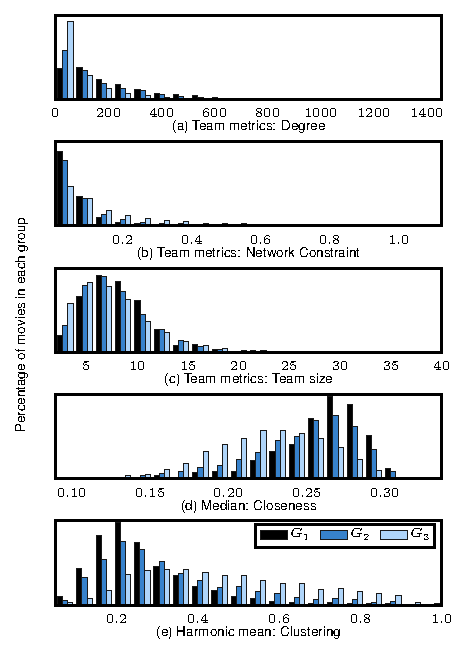
\includegraphics[width=0.78\columnwidth]{../../images/features_hist_top.pdf}
\caption{\label{fig:hist_feat_top}Distribution of topological features for
movies in the three different performance groups. The $x$ axis represents the
portion of movies from the given group (encoded by color) having the specified
value.}
\end{center}\end{figure}


\begin{figure}[H]\begin{center}
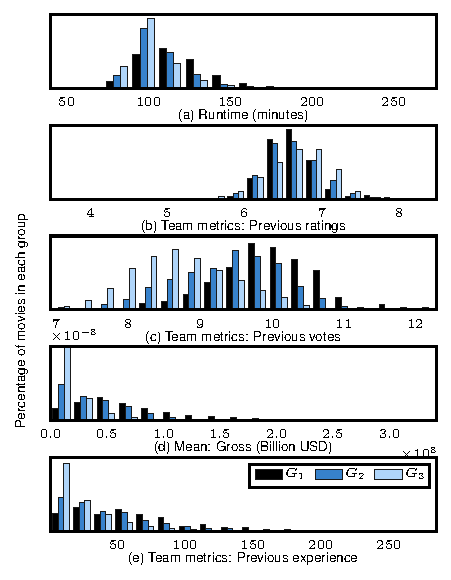
\includegraphics[width=0.78\columnwidth]{../../images/features_hist_ntop.pdf}
\caption{\label{fig:hist_feat_ntop}Distribution of non topological features for
movies in the three different performance groups. The $x$ axis represents the
portion of movies from the given group (encoded by color) having the specified
value.}
\end{center}\end{figure}

\subsection{Producing Successful Movies}
\label{sec:future}
In this section, we assume new teams showing topological characteristics
previously associated to successful movies have a higher probability of
producing successful movies. Under this assumption, we present how our findings
can help to chose agents for a new movie producing team, such that it has
improved success odds.

Figures~\ref{fig:hist_feat_top}~and~\ref{fig:hist_feat_ntop} show movies that
perform better are well determined by their features ranges.  We believe new
teams whose characteristics fall in the same range of values as other
successful teams would be more likely to succeed as well. For example, from
Figure~\ref{fig:hist_feat_top}, movies from the $G_1$ group (blockbusters) are
more likely to have a low clustering coefficient (0--0.3 interval) when
compared to $G_2$ and $G_3$. Moreover, successful teams are likely to have
degree larger than 100, network constraints smaller than 0.1, team sizes of
6--10 people, and closeness greater than 0.25.

We observe that teams with a combined past
experience of 50+ movies are more likely to produce highly successful movies.
Also, teams whose previous movies got an average mean gross of USD 50 million
have a higher chance of producing successful movies. We also see that the mean
rating from movies produced by team members should not deviate much from the
global mean (6--7). Ideally, one should pick producers whose previous
movies received in average about $8,000$ votes.

\section{Results}
\label{sec:results}
In this chapter, we present an experimental evaluation for our prediction
model. First, the prediction model is evaluated with three different groups of
features (Section~\ref{sec:chronological}). The most and least successful
movies are presented along with their team's key topological features
(Section~\ref{sec:bestworst}). We then present the movies of different levels
of success for which the predicted values had greatest and smallest prediction
errors (Section~\ref{sec:hitsmisses}). Finally, we conclude this section by
taking all results together and giving insights into ways of producing a
blockbuster (Section~\ref{sec:an:final}).

\subsection{Prediction Model Evaluation}
\label{sec:chronological}
Here, we evaluate the three instances of regression models for predicting each
of the three success parameters based on each chronological test set
(Table~\ref{tab:test_sets}). Table~\ref{tab:years_results} presents $R^2$
measures for each model instance. The model that only uses non-topological
features is taken as baseline because it only uses features already explored by
previous works (e.g., genre, runtime, and budget).

\definecolor{Gray}{gray}{0.85}
\newcolumntype{a}{>{\columncolor{Gray}}r}
\newcolumntype{b}{>{\columncolor{Gray}}c}

\begin{table}[tb]
\caption{\label{tab:years_results}Coefficient of determination ($R^2$) and
confidence intervals for a significance level of $95\%$ obtained with a
Bayesian Ridge regression for different configurations of year range of the
dataset, and features employed in the regression.}
\centering
\begin{tabular}{lcccba}
\toprule
Target                  & Years      & Non Topol.    & Topologic & All & Gain \\
\midrule
\multirow{3}{*}{Votes}  & 2008--2013   & $.529$, {\tiny $\pm$}$.0008$ & $.310$, {\tiny $\pm$}$.0006$ & $.556$, {\tiny $\pm$}$.0008$ & $5.10\%$ \\
                        & 2000--2013   & $.484$, {\tiny $\pm$}$.0004$ & $.294$, {\tiny $\pm$}$.0005$ & $.517$, {\tiny $\pm$}$.0004$ & $6.82\%$ \\
                        & 1990--2013   & $.437$, {\tiny $\pm$}$.0003$ & $.246$, {\tiny $\pm$}$.0004$ & $.464$, {\tiny $\pm$}$.0003$ & $6.18\%$ \\
\midrule
\multirow{3}{*}{Gross}  & 2008--2013   & $.431$, {\tiny $\pm$}$.0008$ & $.170$, {\tiny $\pm$}$.0013$ & $.448$, {\tiny $\pm$}$.0009$ & $3.94\%$ \\
                        & 2000--2013   & $.419$, {\tiny $\pm$}$.0004$ & $.175$, {\tiny $\pm$}$.0005$ & $.447$, {\tiny $\pm$}$.0004$ & $6.68\%$ \\
                        & 1990--2013   & $.392$, {\tiny $\pm$}$.0004$ & $.174$, {\tiny $\pm$}$.0004$ & $.435$, {\tiny $\pm$}$.0003$ & $10.97\%$ \\
\midrule
\multirow{3}{*}{Rating} & 2008--2013   & $.271$, {\tiny $\pm$}$.0011$ & $.033$, {\tiny $\pm$}$.0009$ & $.281$, {\tiny $\pm$}$.0012$ & $3.69\%$ \\
                        & 2000--2013   & $.267$, {\tiny $\pm$}$.0006$ & $.038$, {\tiny $\pm$}$.0003$ & $.273$, {\tiny $\pm$}$.0006$ & $3.37\%$ \\
                        & 1990--2013   & $.258$, {\tiny $\pm$}$.0004$ & $.031$, {\tiny $\pm$}$.0003$ & $.262$, {\tiny $\pm$}$.0005$ & $1.55\%$ \\
\bottomrule
\end{tabular}
\end{table}


The results show considering a wider range of years in the dataset
\textit{decreases} the effectiveness of the prediction model. We speculate that
it happens because the organization of movie producing teams is constantly
evolving. Hence, forms of organization that were related to best results in one
chronological context might not generalize across all history. As an evidence,
Figure~\ref{fig:features_dist_top} showed a rise of the clustering coefficient
until late 1940's, then a decrease until the mid-1960's, with a very slow
growth until 2013 (Section~\ref{sec:feature_char}). This result strengthens the
importance of splitting the data into different profiles and analysing then
separately.

Also, the model performs very differently when predicting each success
parameter: it performs better for number of votes, a little worse for gross
($R^2$ values are $19.42\%$ smaller than the best model's) and worse still for
normalized ratings ($R^2$ values are $49.46\%$ smaller than the best model's).
Here, we argue that the absolute number of votes a movie receives is the less
noisy variable out of the three.  In other words, more external factors
interfere with gross and ratings. For instance, gross is directly connected to
the audience that \textit{pays} to watch the movie in theaters shortly after the
release. That can be affected by the movie's distribution efficiency and
advertising reach (and the spread of movie piracy). Ratings way be heavily
affected by the performance of a specific actor and the cultural/emotional
response from the audience. The absolute number of votes measures the public
\textit{attention} captured by the movie, since a person may watch and rate it
without necessarily having to pay for it or like it. Finally, such a broad
range of results highlight (once more) that movie success prediction is a
difficult task. It is especially hard when assessing gross and ratings due to
the morphing complexity of production team organization in the movie industry.

Nonetheless, for all cases, the prediction model that considers topological
features (along with past success, past experience and movie characteristics)
outperforms the others. This makes clear topological features do have
predictive power over movie success parameters. Indeed, we see that
topological features \textit{alone} could still be used to train movie success
regression models with better results than pure guesswork.

\begin{figure}[H]\begin{center}
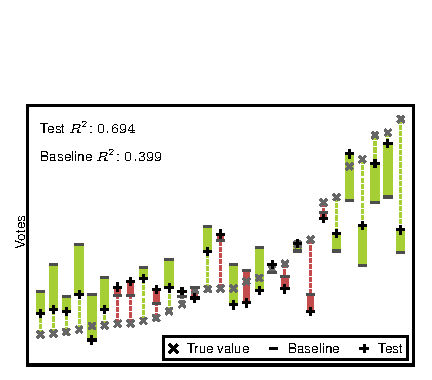
\includegraphics[width=0.9\columnwidth]{../../images/pred_final2.pdf}
\caption{\label{fig:pred_evaluation}Performance comparison of regression
models without (baseline) and with (test) topological features, using the same
movie train/test split. Green bars for when test is better than baseline, and
red bars otherwise.}
\end{center}\end{figure}

\subsubsection{Topological Features Influence}
In order to complement our discussion, Figure~\ref{fig:pred_evaluation} is a
graphic comparison between using only non-topological features (baseline) and
using all features (test). This evaluation considers a random sample of 29
movies\footnote{This is just an \textbf{illustrative} sample of how our predictor
compares to the baseline. The sample has only 29 movies for clarity reasons.}.
Both models were trained and tested with the chronological dataset
[2008--2013]–which produced the best results (Section~\ref{sec:chronological}).
The $y$ axis is scaled to the $[0,1]$ interval. In order to improve
readability, movies in the test set are ordered by their predicted
variable magnitude (ground truth), i.e.\@ the movie's actual
\textit{$\log\kern\nulldelimiterspace(\textrm{number of votes})$}.

This extra analysis emphasizes the relevance of considering network topology. 
In fact, we may claim that it ushers the development of
more sophisticated prediction models in which the \textit{topology} of teams is
also considered. Moreover, new tools could unveil new knowledge on how precisely the
network topology impacts team success in broader contexts.

\subsubsection{``Super''-Regressor}
In this final evaluation, we study how including success parameters into the
set of 23 features (Table~\ref{tab:selected_features}) can improve prediction
accuracy.  Specifically, given one success parameter, we include the other two
in the feature set. For instance, this would be helpful when having two
parameters already computed (even if partially) and trying to predict the third
one.  Considering that we want to predict the number of votes, using all
selected features plus movie ratings and gross gives a Bayesian Ridge
regression with $R^2 = 0.670$, confidence interval~$= 0.0007$ and
$\alpha=95\%$. Using the same strategy, we can predict gross with $R^2 =
0.573$, confidence interval~$= 0.0013$, and $\alpha=95\%$. For ratings, the
results are $R^2 = 0.356$, confidence interval~$= 0.0013$, and $\alpha=95\%$. A
side by side comparison of the best performing model against the one with
these extra features is shown Table~\ref{tab:years_results_super}. Using just
one extra feature yields results that are worse when two extra features
are used. However, even when just one extra feature is used, the results are
still better when compared to the best perming model that does not use
pre-release information.  Finally, these results hint an even better prediction
model might be obtained for long-term success of movies considering their
initial success.

\definecolor{Gray}{gray}{0.85}
\newcolumntype{a}{>{\columncolor{Gray}}r}
\newcolumntype{b}{>{\columncolor{Gray}}c}

\begin{table}[tb]
\caption{\label{tab:years_results_super}Coefficient of determination ($R^2$) and
confidence intervals for a significance level of $95\%$ obtained with a
Bayesian Ridge regression. It shows the best results obtained only using
pré-release information side by side with results obtained when also using
other of the movie's success parameters as new features.} 
\centering
\begin{tabular}{lccr}
\toprule
Target                  & Years      & Without extra features    & With extra features \\
\midrule
\multirow{3}{*}{Votes}
& 2008--2013   & $.556$, {\tiny $\pm$}$.0008$ & $.670$, {\tiny $\pm$}$.0007$ \\
& 2000--2013   & $.517$, {\tiny $\pm$}$.0004$ & $.687$, {\tiny $\pm$}$.0004$ \\
& 1990--2013   & $.464$, {\tiny $\pm$}$.0003$ & $.669$, {\tiny $\pm$}$.0004$ \\
\midrule
\multirow{3}{*}{Gross}
& 2008--2013   & $.448$, {\tiny $\pm$}$.0009$ & $.574$, {\tiny $\pm$}$.0009$ \\
& 2000--2013   & $.447$, {\tiny $\pm$}$.0004$ & $.613$, {\tiny $\pm$}$.0006$ \\
& 1990--2013   & $.435$, {\tiny $\pm$}$.0003$ & $.614$, {\tiny $\pm$}$.0005$ \\
\midrule
\multirow{3}{*}{Rating}
& 2008--2013   & $.281$, {\tiny $\pm$}$.0012$ & $.438$, {\tiny $\pm$}$.0014$ \\
& 2000--2013   & $.273$, {\tiny $\pm$}$.0006$ & $.479$, {\tiny $\pm$}$.0007$ \\
& 1990--2013   & $.262$, {\tiny $\pm$}$.0005$ & $.480$, {\tiny $\pm$}$.0006$ \\
\bottomrule
\end{tabular}
\end{table}


\subsection{Best and Worst Movies}\label{sec:bestworst}
For better illustrating the analysis, we present the best and worst movies
according to the normalized mean of the success factors.
Tables~\ref{tab:worst_movies}~and~\ref{tab:best_movies} respectively show the
movies with the highest and lowest scores, including examples of low-scoring
popular movies and high-scoring unpopular movies.

\begin{table}[tb]
\caption{\label{tab:worst_movies}Worst movies by normalized average of ratings, gross revenue and number of votes. The last two are low scoring movies that are also popular (received more than 6 thousand votes).}
\centering
\begin{tabular}{lrrrr}\toprule
Movie Title                    & Score & Degree & Team Size & Clustering      \\ \midrule
Waxwork II:\@ Lost in Time (1992) & .247      & 32     & 2         & .296   \\
Fuk sau che chi sei (2010)     & .252      & 3      & 2         & 1.00        \\
Nature Calls (2012)            & .259      & 77     & 5         & .322      \\
Perro come perro (2008)        & .264      & 17     & 7         & .796   \\
Playback (II) (2012)           & .269      & 309    & 12        & .332   \\
Jack \& Diane (2012)           & .269      & 95     & 11        & .419   \\
Angels Crest (2011)            & .291      & 71     & 5         & .371   \\
Che? (1972)                    & .299      & 15     & 4         & .185  \\ \midrule
S. Darko (2009)                & .306      & 109    & 7         & .402    \\
Captain America (1990)         & .331      & 97     & 5         & .200      \\ \bottomrule
\end{tabular}
\end{table}

\begin{table}[tb]
\caption{\label{tab:best_movies}Best movies by normalized average of ratings,
gross revenue and number of votes. The last three are high-scoring movies that
are also not very popular (received less than 5 thousand votes).}
\centering
\begin{tabular}{lrrrr}\toprule
Movie Title                     & Score      & Degree & Team Size & Clustering  \\ \toprule
The Dark Knight (2008)          & .978      & 343    & 10        & .275   \\
The Lord of the Rings (2003)    & .952      & 77     & 5         & .251   \\
Inception (2010)                & .949      & 17     & 7         & .176   \\
The Lord of the Rings (2001)    & .946      & 309    & 12        & .252   \\
The Lord of the Rings (2002)    & .941      & 95     & 11        & .228   \\
Star Wars (1977)                & .94       & 71     & 5         & .264   \\
The Dark Knight Rises (2012)    & .938      & 15     & 4         & .176   \\
Pulp Fiction (1994)             & .936      & 5      & 10        & .195   \\
The Shawshank Redemption (1994) & .936      & 109    & 7         & .241   \\
The Matrix (1999)               & .934      & 97     & 5         & .218   \\ \midrule
Friendly Persuasion (1956)      & .599      & 9      & 4         & .180   \\
They Drive by Night (1940)      & .599      & 17     & 2         & .263   \\
Hubble 3D (2010)                & .580      & 3      & 3         & .208   \\ \bottomrule
\end{tabular}
\end{table}


These results confirm our findings: for bad movies, all values of team harmonic
mean of clustering coefficient are below $0.280$, whereas good movies obtained
higher values. Degree and team size values for movies are comparable across the
two tables. However, as seen in
Sections~\ref{sec:featureselection}~and~\ref{sec:future}, these metrics play a
very important part in the regression model if combined with other features.
This might indicate that these features provide predictive power once combined
with other features.

\subsection{Prediction Hits and Misses}
\label{sec:hitsmisses}
In this section, we dissect the prediction results by calculating the
difference between predicted values and real values of success parameters for
each movie. Specifically, we predict movie's success parameters 30 different
times (using the same methodology previously presented), and store the
predicted results. We use these predictions to compute the mean prediction
error and confidence interval associated with success parameters for each
movie.

By using these values, we focus our analysis on the movies in which our model
predicts success parameters with highest and lowest errors, i.e., our
prediction misses and hits. To provide a throughout overview of such movies, we
present a separate table for displaying errors from prediction results in each
of the three success parameters. Each table is also divided in two parts, one
shows nine movies with high prediction error (misses), and the other shows nine
movies with low prediction errors (hits). Also, in each table, rather than
showing the movies having the overall highest and lowest errors, we select nine
movies having success values from distinct ranges: $0$--$0.2$, $0.2$--$0.3$,
$0.3$--$0.4$ and so on until the range $0.9$--$1.0$. Considering all movies
that would fit the range, the movie having the highest (or lowest) prediction
error is displayed on the table. In other words, the movies in these tables
were selected by picking the highest (or lowest) prediction error for the
movies having different ranges of the success parameter being observed in the
table.

According to this organization,
Tables~\ref{tab:errors_pred_gross},~\ref{tab:errors_pred_votes}
and~\ref{tab:errors_pred_rating} show the predictor's hits and misses for
gross, number of votes and ratings. All values (but degree) are normalized for
clarity. Each table is ordered by the level of success of the movie according
to the table's success parameter (i.e., Table~\ref{tab:errors_pred_gross}
ordered by gross, Table~\ref{tab:errors_pred_votes} ordered by vote, and
Table~\ref{tab:errors_pred_rating} by rating), from the weakest to the
strongest. Two topological characteristics are also highlighted: clustering and degree
(which could explain some of the hit and misses, Section~\ref{sec:featureselection}).

We now take a closer look at some of those movies starting with \textit{Erased}
(2012) in Table~\ref{tab:errors_pred_gross}.  It had an estimated budget of 12
million euros and was produced by an experienced team of producers. Such
features lead our predictor to assign a high gross value to it.  However, the
movie gross extracted from IMDb database is very low (only 147 British pounds),
resulting in a high prediction error. Hence, either it is a really unexpected
outcome, or there is a typo in the gross data.

On the other hand, consider the movie \textit{Hubble 3D}
(2010), for which the model heavily under-predicted the gross income. Its
producers had very little past experience or past success, and they were very
poorly connected to other producers in the network. This indicated the movie would
be a good candidate for a flop. However, it was one of the first feature-length IMAX
productions, whose work was overseen by IMAX itself. With such innovative
aspects, it drew masses to movie theaters.

\begin{table*}[!t]
\caption{\label{tab:errors_pred_gross}Errors in predictive results for gross.}
\centering

\begin{subtable}[b]{\textwidth}
\caption{\textbf{Predictor Misses}}
\centering
\begin{tabular}{lrrrr} \toprule
Title                       & Clustering & Degree & Error  & Gross \\ \midrule
Erased (2012)               & .290       & 352    & +.489  & .148  \\
Loosies (2011)              & .451       & 232    & +.416  & .293  \\
Leap Year (2010)            & .118       & 574    & +.518  & .370  \\
Ballast (2008)              & .303       & 109    & +.457  & .475  \\
In the Land of Blood (2011) & .252       & 204    & +.324  & .550  \\
The Objective (2008)        & .433       & 224    & -.235  & .668  \\
You're Next (2011)          & .446       & 43     & -.304  & .783  \\
Hubble 3D (2010)            & .857       & 3      & -.366  & .843  \\
Slumdog Millionaire (2008)  & .174       & 303    & -.284  & .904  \\ \bottomrule
\end{tabular}
\end{subtable}

\vspace*{.5 cm}

\begin{subtable}[b]{\textwidth}
\caption{\textbf{Predictor Hits}}
\centering
\begin{tabular}{lrrrr} \toprule
Title                    & Clustering & Degree & Error & Gross \\ \midrule
Emergo (2011)            & .836       & 5      & +.298 & .147  \\
London River (2009)      & .344       & 74     & +.137 & .241  \\
The ABCs of Death (2012) & .718       & 149    & -.003 & .399  \\
From Within (2008)       & .854       & 6      & -.002 & .468  \\
Cheung Gong 7 (2008)     & .382       & 76     &  .000 & .532  \\
Cocktail (2012)          & .447       & 62     &  .000 & .620  \\
Haywire (2011)           & .096       & 562    &  .000 & .785  \\
Predators (2010)         & .202       & 211    &  .000 & .846  \\
Ice Age: Dawn of (2009)  & .797       & 7      & +.001 & .923  \\ \bottomrule
\end{tabular}
\end{subtable}

\end{table*}

\begin{table*}[!t]
\caption{\label{tab:errors_pred_votes}Errors in predictive results for votes.}

\begin{subtable}[b]{\textwidth}
\caption{\textbf{Predictor Misses}}
\centering
\begin{tabular}{lrrrr} \toprule
Title                   & Clustering & Degree & Error  & Votes \\ \midrule
The Incident (2011)     & .152       & 161    & +.358  & .132  \\
The Factory (2012)      & .147       & 554    & +.431  & .254  \\
Recep Ivedik (2008)     & .540       & 6      & -.297  & .372  \\
Black Dynamite (2009)   & .929       & 10     & -.393  & .479  \\
ParaNorman (2012)       & .820       & 7      & -.505  & .570  \\
Yip Man (2008)          & .709       & 24     & -.546  & .663  \\
Moon (2009)             & .565       & 104    & -.561  & .742  \\
Intouchables (2011)     & .699       & 10     & -.633  & .813  \\
Django Unchained (2012) & .079       & 984    & -.115  & .905  \\ \bottomrule
\end{tabular}
\end{subtable}

\vspace*{.5 cm}

\begin{subtable}[b]{\textwidth}
\caption{\textbf{Predictor Hits}}
\centering
\begin{tabular}{lrrrr} \toprule
Title                     & Clustering & Degree & Error & Votes  \\ \midrule
Buck (2011)               & .511       & 68     &  .000 & .119   \\
Zweiohrküken (2009)       & .312       & 82     &  .000 & .221   \\
Wrecked (2010)            & .272       & 421    & +.001 & .337   \\
Cyrus (2010)              & .201       & 167    & -.001 & .460   \\
Don't Be Afraid of (2010) & .169       & 348    &  .000 & .502   \\
The Last Airbender (2010) & .230       & 211    &  .000 & .642   \\
Fast Five (2011)          & .190       & 222    & -.003 & .753   \\
X-Men: First Class (2011) & .205       & 361    & -.009 & .833   \\
The Dark Knight (2008)    & .202       & 343    & -.035 & .996   \\ \bottomrule
\end{tabular}
\end{subtable}

\end{table*}

\begin{table*}[!t]
\caption{\label{tab:errors_pred_rating}Errors in predictive results for ratings}

\begin{subtable}[b]{\textwidth}
\caption{\textbf{Predictor Misses}}
\centering
\begin{tabular}{lrrrr}
\toprule
Title                           & Clustering & Degree & Error  & Rating \\ \midrule
Jonas Brothers: The 3D (2009)   & .466       & 149    & +.551  & .137   \\
Hannah Montana \& Miley (2008)  & .880       & 16     & +.484  & .228   \\
Zeiten ändern Dich (2010)       & .221       & 148    & +.339  & .341   \\
Utomlyonnye solntsem 2 (2010)   & .763       & 24     & +.314  & .481   \\
Mausam (2011)                   & .564       & 26     & +.209  & .509   \\
Cars 2 (2011)                   & .600       & 4      & +.296  & .622   \\
Zombieland (2009)               & .130       & 272    & -.301  & .790   \\
How to Train Your Dragon (2010) & .278       & 183    & -.257  & .855   \\
The Dark Knight (2008)          & .202       & 343    & -.253  & .961   \\ \bottomrule
\end{tabular}
\end{subtable}

\vspace*{.5 cm}

\begin{subtable}[b]{\textwidth}
\caption{\textbf{Predictor Hits}}
\centering
\begin{tabular}{lrrrr}
\toprule
Title                           & Clustering & Degree & Error & Rating \\
\midrule
Dragonball Evolution (2009)     & .281       & 105    & +.422 & .174   \\
Far Cry (2008)                  & .298       & 165    & +.240 & .295   \\
BloodRayne: The Third (2011)    & .304       & 141    & +.123 & .367   \\
It's Alive (2009)               & .134       & 850    & +.012 & .487   \\
Livide (2009)                   & .321       & 33     &  .000 & .598   \\
Scusa ma ti chiamo amore (2008) & .076       & 18     &  .000 & .641   \\
No One Killed Jessica (2011)    & .327       & 112    & +.001 & .717   \\
Gangs of Wasseypur (2012)       & .459       & 92     & -.005 & .889   \\
The Dark Knight Rises (2012)    & .198       & 372    & -.168 & .908   \\
\bottomrule
\end{tabular}
\end{subtable}

\end{table*}


Now, consider the movie \textit{Ice Age: Dawn of the Dinosaurs} (2009) as one
big hit. Even though it has a very high clustering coefficient, the model still
predicted its gross almost to the point (error of $+.001$). Such result shows
its team's past success (in gross) was high enough to counterbalance the team's
high heterogeneity. Likewise, we note that among the hits, the highest errors
are within the low performance group ($G_3$ with \textit{Emergo} and
\textit{London River}).

Table~\ref{tab:errors_pred_votes} presents some interesting results while
predicting movie popularity (number of votes). For instance, the movie
\textit{Intouchables} (2011) was produced in France by an unexperienced
producing team whose past productions were unpopular or obscure movies. None of
the producers had ever produced a single movie that had reached such a mass
success. However, this movie has a widely acclaimed high-quality storyline. So,
even though it had a relatively low gross, barely covering its budget, the
movie name spread after its release, reaching a wide level of popularity.

For the hits on this table, we note the high performance group has only movies
from big franchises: \textit{Fast Five}, \textit{X-Men: First Class} and
\textit{The Dark Knight}. Given that franchises tend to keep their producing
teams fairly large and well connected, it also provides more interesting
team-based features for the predictor to hit the mark.

Table~\ref{tab:errors_pred_rating} presents the predictor hits and misses for
ratings, whose errors are more evident than the previous parameters. The main
reason here could be cultural factors. For instance, movies like \textit{Jonas
Brothers} (2009) and \textit{Hanna Montana \& Miley Cyrus} (2008) which are
about teenage pop singers, received extremely low ratings. Nonetheless, these
movies were produced by experienced and well connected teams with the support
of a huge producing company (Walt Disney Pictures), have extremely popular
actors/singers and made significant box offices. It is possible that the
ratings came from the kids' parents and not the kids themselves, who would
probably rate them as an award quality movie. Such cultural aspects are very
hard (if not impossible) to detect from movie topology or other concrete movie
features considered here.

The hits on Table~\ref{errors_pred_ratings} are probably the hardest to
explain. Nonetheless, as for the misses, we postulate the cultural aspects
involved in these movies could also explain such results. Moreover, the
profiles of the three top performance movies are completely different:
\textit{No one Killed Jessica} is an India-produced crime-drama-thriller;
\textit{Gangs of Wasseypur} is an R-rated Indian 320-minute movie featured at
Cannes Film Festival; and \textit{The Dark Knight Rises} ends Christopher
Nolan's Batman trilogy.

\subsection{Final Considerations}
\label{sec:an:final}
In this chapter, we have confirmed that it is indeed possible to predict
success by considering only data available \textit{before} the movie is
released. Also, considering a large dataset for the prediction task is good;
however, spanning it through many years may negatively affect the quality of
the regression models. Finally, for all cases, the prediction model with
topological features combined with past success and experience have
outperformed the others, confirming this work main hypothesis.

Besides identifying the most relevant features, it is also important to assess
their \textit{strength} by evaluating their coefficients in the regression
model. Note that features with a higher coefficient have more impact in the
predicted value. Hence, we take an already trained regression model (the one
for votes, whose fitting was the best among the three parameters) and sort its
coefficients in descending magnitude. The coefficients with the highest
magnitudes are: the team's mean previous gross, mean previous experience, the
harmonic mean of clustering coefficients, contracted degree, genres Drama and
Documentaries, runtime and continent Africa. 

Out of all topological features, the impact of the \textit{clustering
coefficient} and \textit{degree} are significantly higher than the others
(their actual values are informed in the illustrative samples on the hits and
misses analyzes in Section~\ref{sec:hitsmisses}). Also, teams with more ties to
producers outside the current team are more likely to succeed, as are teams
with the lowest levels of clustering coefficients. These indicate that more
homogeneous teams tend to perform worse. In other words, this is a very
important result and suggests that assembling heterogeneous teams with many
\textit{external connections} is key in forming a team with higher success
odds. It is important to notice that such results reinforce the theory of weak
ties (or structural holes) that determine the importance of having nodes acting
as \textit{bridges} within a successful
network~\citep{Burt04,burt2005brokerage,newman2001structure}.

